\documentclass[12pt,twoside]{article}
\input{.house-style/preamble.tex}
\setlength{\headheight}{14pt}
\setlength{\emergencystretch}{2em}
\clubpenalty=10000
\widowpenalty=10000
\brokenpenalty=10000
\setcounter{topnumber}{1}

\hypersetup{
  pdftitle={What Generalizes in Reliability Generalization?},
  pdfkeywords={reliability generalization, measurement error, task engagement, estimands, research synthesis}
}

\title{What Generalizes in Reliability Generalization?}
\author{Brett Reynolds \orcidlink{0000-0003-0073-7195}%
\thanks{Contact: \href{mailto:brett.reynolds@humber.ca}{brett.reynolds@humber.ca}}\\
Humber Polytechnic \& University of Toronto}
\date{Preprint, November 2026}

\begin{document}
\maketitle

\begin{abstract}
Zhao and Plonsky's synthesis of task-engagement research uses a distribution of reported reliability coefficients to assess measurement quality and discuss minimum acceptability. Such judgments require more than a position in that distribution. As the authors note, the pooled coefficients don't all summarize the same measurement property, and even comparable coefficients have different consequences for different scientific targets. Using the synthesis as a worked case, this response connects the authors' cautions about coefficient choice to their rationale for a percentile benchmark. Under explicit classical-error models, reliability of .6 leaves a randomized raw mean contrast unbiased but reduces its effective sample size to 60\% of the original. An uncorrected slope on a noisy predictor instead converges to 60\% of the latent slope. Standardized differences and correlations require further distinctions. These familiar results show why a field percentile alone can't tell a researcher what a planned study can learn. A worked planning example shows how, under the stated model, reliability and sample size together set the precision of an experimental contrast. Reliability syntheses can better support such decisions by displaying comparable coefficients separately and connecting them to uncertainty about specified estimates and predictions.
\end{abstract}

\noindent\textbf{Keywords:} reliability generalization; measurement error; task engagement; estimands; research synthesis
\aidisclosure{GPT-6 (\texttt{gpt-6-astra} in OpenAI Codex, and in ChatGPT for an external review), Claude Opus 5.5, and ChatGPT (original-brief model unrecorded)}

\section{What does a reliability benchmark justify?}

A researcher needs to decide whether an engagement measure is adequate for a planned study. Knowing where its reliability coefficient falls among published values provides context. It doesn't yet say how much measurement error would change the study's conclusion. Assessing what a planned study can learn requires connecting measurement error to uncertainty about its intended estimates or predictions.

\textcite{ZhaoPlonsky2026} make the issue concrete. Their synthesis reports a median of .89 across 111 coefficients from 30 studies, and they take this to suggest that the measures are \enquote{overall, quite reliable} (p.\ 1). They stress that the primary purpose of such a synthesis \enquote{is not to simply establish an average level or threshold of reliability, but to examine the variation of reliability across samples and contexts} (p.\ 2). They also repeat a qualified recommendation from \textcite{PlonskyDerrick2016}: the 25th percentile for each type of reliability can serve as a general minimum benchmark, and results below it call for caution because \enquote{measurement error may attenuate observed effects} \citep[p.\ 7]{ZhaoPlonsky2026}.

\textcite[p.\ 550]{PlonskyDerrick2016} present such type-specific percentiles as an improvement on \enquote{arbitrary and binary acceptable/nonacceptable labels}, and they ask that attenuation be \enquote{taken into consideration, whether in the form of psychometric corrections or simply in prose} (p.\ 548). Both points are right: standing among comparable studies says more than a fixed cutoff, and error can attenuate effects.

The missing step is why a particular percentile marks an acceptable consequence for the research question. Error can reduce precision, change a standardized effect, bias an uncorrected estimate of a latent relation, or impair prediction. A coefficient's rank among published values can prompt investigation, but it determines neither the presence nor the size of these consequences. Researchers need the quantity to be estimated~-- the \term{estimand}~-- and an account of how measurement enters its estimation.

Two questions follow. Do the coefficients being compared concern the same measurement property? If they do, what does that property imply for the intended inference? Zhao and Plonsky recognize several limits relevant to the first question: they distinguish reliability from validity, acknowledge sample dependence, and warn against interpreting differences among indices as differences in measurement quality (pp.\ 6, 10). Their inventory is useful, especially its finding that task-specific reliability is often unavailable. The response below applies those cautions to the synthesis's subgroup interpretations and then addresses the second question.

\section{Do the coefficients support the comparison?}

Earlier work co-authored by Plonsky provides a diagnostic for interpreting subgroup differences. \textcite[p.\ 549]{PlonskyDerrick2016} found higher reliability among instruments not reported as piloted and pointed to coefficient choice as an explanation: the groups used different mixtures of indices. \textcite[p.\ 252]{ZhaoPlonsky2024} give a related caution: a benchmark based largely on alpha (an index of consistency among items) may not apply to omega (a reliability estimate derived from a factor model). These cautions call for checking what coefficients measure before treating their numerical values as evidence of measurement quality.

That check is consequential in the task-engagement synthesis. On pp.\ 9--10, \textcite{ZhaoPlonsky2026} describe higher medians for observation and interaction than for Likert-type scales, and connect this pattern to the gap between interrater and internal-consistency coefficients. They suggest that the pattern \enquote{likely reflects} differences between observable and latent engagement; self-report could introduce \enquote{additional sources of measurement error}. But the note to their Table~2 says that the combined summaries \enquote{aggregate indices with different measurement meanings} and that numerical differences across indices \enquote{should not be interpreted as differences in measurement quality} (p.\ 6). On p.~10 they add that the coefficient-type differences in Tables~3 and~4 \enquote{are more likely to be attributed to the statistical properties of the coefficients than to instrument quality}.

Consider the related comparison by measurement source. As printed in their Table~4, 44 of the 57 self-report estimates are alpha coefficients. The 44 researcher-observation estimates include 13 Pearson correlations and 18 agreement percentages \citep[p.\ 8]{ZhaoPlonsky2026}. Such summaries don't separate differences in measurement quality from differences in what the indices summarize. The proposed explanation might be right, but the combined medians don't establish it.

Zhao and Plonsky's Table~4 reports medians of .94 during the task and .87 immediately afterward. The during-task group contains all 17 Pearson correlations and 24 of 25 agreement percentages; the post-task group contains 43 of 46 alpha coefficients. The authors tentatively attribute the contrast to observable behaviour versus retrospective self-report (p.\ 10). That explanation already ties timing to the scored object; coefficient choice is entangled with both.

These figures follow Table~4 as printed. Zhao and Plonsky's Table~2 reverses the Pearson/agreement counts, medians, and interquartile ranges. A simple swap of those labels would preserve their combined concentration in the during-task group and the predominance of alpha afterward. It wouldn't reconcile the extraction or establish corrected medians; the discrepancy still limits numerical reanalysis.

Three constructed examples, each containing four paired observations, illustrate what different summaries retain. Suppose two observers count events in the same four clips, with observer A reporting $(1,2,3,4)$. Neither observer is designated as correct. Table~\ref{tab:correlation-agreement} varies B's counts: a one-count shift preserves perfect correlation while removing every exact match; reversing the order gives correlation $-1$ with the same zero agreement.

\begin{table}[tbp]
\centering
\caption{Three constructed examples with A fixed at $(1,2,3,4)$. These are event counts, not codes for nominal categories.}
\label{tab:correlation-agreement}
\begin{tabular}{@{}lcc@{}}
\toprule
B's counts & Pearson $r$ & Exact agreement \\
\midrule
$(1,2,3,4)$ & $1$ & $4/4$ (100\%) \\
$(2,3,4,5)$ & $1$ & $0/4$ (0\%) \\
$(4,3,2,1)$ & $-1$ & $0/4$ (0\%) \\
\bottomrule
\end{tabular}
\end{table}

Correlation summarizes linear covariation and is unchanged by shifting or positively rescaling either series; exact agreement records equality and discards the size of each mismatch. An online interactive supplement (\url{https://brettreynolds.ca/correlation-and-agreement/}) lets readers edit the counts, follow both calculations, and construct examples compatible with a given summary. These possibilities establish no empirical frequencies in engagement research.

\section{What's being generalized?}

Grouping by coefficient name is insufficient. Zhao and Plonsky's Table~4 reports alpha under both internal consistency (41 coefficients, median .83) and interrater/coder reliability (five, median .97). Repeating items and repeating coders vary different parts of the measurement procedure. Within one family of indices, variants may concern single or averaged ratings, consistency or absolute agreement, and fixed or sampled coders \citep[p.\ 30]{Hallgren2012}.

For engagement, a learner's score on a particular task and that learner's average over a range of tasks are different targets. Variation across tasks distinguishes one task-specific target from another; sampling tasks contributes uncertainty about the cross-task average.

Generalizability theory makes the choice of target, and of the conditions allowed to vary, explicit. A generalizability study estimates variance components over a declared universe of admissible observations; a decision study uses them for a specified measurement procedure and universe of generalization \citep[pp.\ 5--9]{brennan2001generalizability}. \textcite[p.\ 14]{brennan2001generalizability} illustrates how two investigators can use the same components while generalizing over different conditions: one varies both prompts and raters, while the other holds the prompts fixed. Person-by-prompt variation then contributes differently to universe-score and error variance.

A variance-ratio reliability also depends on the population, because it can change with the spread of the measured quantity even when measurement-error variance stays constant \citep[p.\ 24]{Hallgren2012}. The \enquote{reliability paradox} illustrates this dependence: tasks with robust within-person condition effects can leave too little variance between people for reliable individual differences \citep{HedgePowellSumner2018}, a pattern taken up in L2 work on inhibitory control \citep{WuJiaHui2025}.

These are established measurement distinctions. The further question for a reliability synthesis is how its evidence supports a subsequent study using the score. A defensible score-level reliability estimate still needs to be connected to the mean contrast, association, prediction, or decision for which adequacy is being claimed.

\section{What would measurement error change?}

To examine the benchmark's attenuation rationale, suppose an engagement measure has reliability .6 under a classical model with independent, mean-zero error. In a balanced randomized experiment, error of this kind leaves the raw mean contrast unbiased. Its variance equals that of an error-free study with 60\% of the learners. Increasing the sample can compensate for this loss of precision. The reliability coefficient alone doesn't determine how precisely the study can estimate the treatment contrast.

In a second design, engagement predicts learning and the target is the regression slope for latent engagement. Regressing learning on the noisy score with ordinary least squares (OLS) without correcting for measurement error yields a slope that converges to 60\% of that target. More learners concentrate this estimator around the attenuated value. They don't recover the latent slope. These examples use the same numerical reliability under different population conditioning: within treatment arms in the experiment, and across the predictor population in the regression.

Table~\ref{tab:attenuation} distinguishes these results from standardized effects and correlations. A raw mean contrast that stays unbiased can still correspond to a smaller standardized difference because error enlarges the within-arm standard deviation \citep{KarvelisDiaconescu2025}. Likewise, the attenuation factor for a correlation with one noisy variable is $\sqrt{\rho}$, rather than the factor $\rho$ for the unstandardized slope. If both variables have independent classical measurement errors, the population correlation is multiplied by $\sqrt{\rho_X\rho_Y}$ \citep[p.\ 254]{ZhaoPlonsky2024}.

\begin{table}[!htbp]
\centering
\caption{Consequences of classical measurement error under the models in Appendix~\ref{app:models}. Here $\rho$ denotes reliability in the corresponding model; factors compare each quantity with its error-free counterpart.}
\label{tab:attenuation}
\begin{tabular}{@{}lcc@{}}
\toprule
Quantity & Factor & At $\rho=.6$ \\
\midrule
Expected raw mean contrast & $1$ & $1$ \\
Standard error of raw mean contrast & $1/\sqrt{\rho}$ & $1.29$ \\
Population standardized difference & $\sqrt{\rho}$ & $.77$ \\
Population slope on the noisy predictor & $\rho$ & $.60$ \\
Population correlation, one noisy variable & $\sqrt{\rho}$ & $.77$ \\
\bottomrule
\end{tabular}
\end{table}

These are model consequences, not estimates from engagement research. A reported alpha, correlation, or agreement coefficient isn't automatically either model's reliability parameter. The standardized-difference and correlation rows concern population quantities, not exact expectations of their finite-sample estimators. Systematic or dependent measurement errors can produce different results.

A known relevant reliability removes the model-implied attenuation by rescaling with the appropriate factor. An estimated reliability adds uncertainty and can introduce finite-sample bias; estimating the right parameter doesn't make a ratio unbiased. For the raw mean contrast, the cost is lost precision, which no rescaling of the same observations recovers.

Figure~\ref{fig:consequences} compares each estimator's root mean squared error (RMSE) with its error-free counterpart. RMSE combines sampling variance and squared bias; a ratio above one indicates greater error for the latent target. In the experiment, the penalty is constant at $1/\sqrt{\rho}$ as sample size grows. For the predictor slope, absolute RMSE decreases toward a nonzero bias floor while error-free RMSE tends to zero, so the relative penalty grows. The underlying formulas and chosen effect sizes are in Appendix~\ref{app:models}.

\begin{figure}[tbp]
\centering
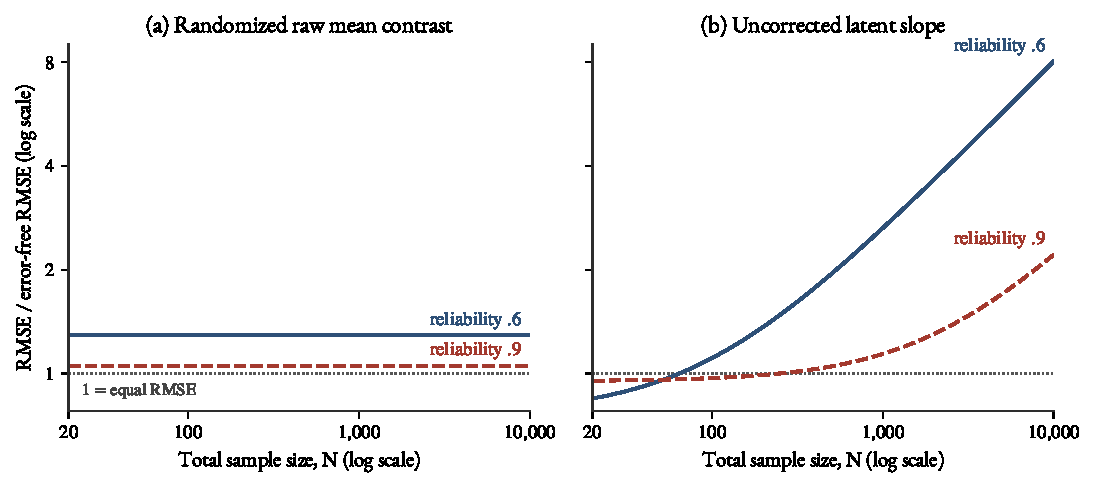
\includegraphics[width=\linewidth]{figures/measurement-consequences.pdf}
\caption{RMSE relative to error-free measurement in each design. Both panels use the same logarithmic scales, and a dotted line at 1 marks equal RMSE. Curves use $\tau=\beta=.2$ and the unit-variance models in Appendix~\ref{app:models}. Panel (b) compares noisy-score OLS with unshrunk error-free OLS.}
\label{fig:consequences}
\end{figure}

Both curves in panel (b) start below one, so at small samples the noisy score gives the lower RMSE. That reflects the estimator as well as the measure. Attenuation shrinks the slope toward zero, which can reduce mean squared error (MSE) relative to unshrunk error-free regression. In this model, applying the same shrinkage to the error-free estimator gives lower MSE than using the noisy score (Appendix~\ref{app:shrinkage}).

Changing the target changes the interpretation again. In the Gaussian predictor model, the attenuated slope is the correct conditional-mean slope for predicting learning from the available noisy score. It's biased for the latent slope but not for that predictive coefficient. Prediction error still depends on measurement quality. An analysis needs to distinguish a relation involving latent engagement from a prediction using the score a future learner will provide.

\textcite[pp.\ 4--6]{PapiSongSoliman2026} report factor-analytic evidence and reliability for the three motivational self-system subscales, and compare motivational constructs as predictors of Intended Effort. One possible latent target is the difference between standardized partial coefficients for Ideal L2 Self and Integrativeness in a joint regression of latent Intended Effort on both latent constructs. This differs from their tested score-level contrasts of unstandardized coefficients. The predictors correlate at .53 (p.\ 5); error in either can bias both coefficients \citep[p.\ 3]{WestfallYarkoni2016}. A joint measurement model could support sensitivity analysis, conditional on which error components the data distinguish and assumptions about the others. Table~\ref{tab:attenuation}'s single-predictor factors don't settle that comparison.

\section{How should adequacy be judged?}

A field percentile alone can't establish adequacy for an intended inference. \textcite[p.\ 548]{PlonskyDerrick2016} qualify their benchmark, distinguish reliability types, and ask researchers to consider stakes. The \textit{Standards for Educational and Psychological Testing} likewise treat \enquote{the minimum acceptable level for any index} as \enquote{a matter of professional judgment} and ask for reliability evidence \enquote{for the interpretation for each intended score use} \citep[pp.\ 41--42]{aera2014standards}.

Even within a comparable class, a percentile changes when reporting practices or the distribution of studies changes. The error consequences for an unchanged study needn't change with it. Standing above the benchmark doesn't establish adequate precision, and standing below it signals the caution Plonsky and Derrick recommend without saying how much an inference is affected.

The practical alternative is to state the inference and examine plausible measurement processes. \textcite[pp.\ 641--643]{gelman2014types} orient design analysis toward what a study can learn about an effect's direction and magnitude, using assumptions informed by more than the observed estimate. Return to the balanced engagement experiment. Its target is the mean treatment contrast in the defined engagement score, expressed in units of its latent within-arm standard deviation.

The relevant reliability concerns variation among learners within treatment arms and error under the intended replication procedure. A pilot with parallel measurements of the same target could inform those components. Under the additive model, the covariance between replicates estimates the latent variance, and half the variance of their difference estimates the error variance (Appendix~\ref{app:models}). This interpretation requires a stable target and equal-variance errors independent of each other and of that target. Shared rater bias or genuine change would require a different model. Without suitable evidence, .6 and .9 are sensitivity scenarios, not estimated reliabilities or established bounds for engagement measures.

With latent within-arm variance set to one, the standard error is $\sqrt{4/(N\rho)}$: about .183 at reliability .6 and .149 at .9 for 200 learners. Under a normal approximation, the corresponding 95\% interval half-widths are about .36 and .29. If the estimated contrast were .2, either interval would include zero. Improving measurement narrows uncertainty without ensuring that this design can determine the direction of a contrast that small. Under the model, 300 learners at reliability .6 provide the same precision as 200 at .9.

These are planning approximations conditional on the stated variances; they don't propagate uncertainty in estimated reliability. Costs and feasibility would be needed to choose between improving measurement and recruiting more learners. The example shows what those choices change under the model, without prescribing an instrument or a sample size.

For a latent-predictor slope, a design analysis could show how estimates change across plausible measurement-error models and carry uncertainty about their parameters through to the estimated slope. Where repeated measurements are available, simulated data from the fitted model can be compared with observed patterns of disagreement across items, raters, or occasions \citep[p.\ 30]{gelman2020bayesianworkflow}. The analysis would clarify what the measurements support about the relation's direction and magnitude. Where a practical decision is involved, the consequences of acting under that uncertainty also need weighing.

A reliability synthesis can support these analyses by recording the scored object, replication design, population, coefficient variant, and intended use, together with study and sample identifiers. Comparable estimates can inform plausible measurement models and their uncertainty. Other estimates remain informative about measurement practice. Hierarchical modelling can accommodate dependence and variation when a defensible common target exists; it doesn't create that target.

Alongside medians and interquartile ranges, syntheses should display individual coefficients within groups sharing a coefficient variant and replication design. REGEMA, a reporting checklist for reliability generalization studies, already asks for separate meta-analyses \enquote{for each type of reliability coefficient} and for graphs of their distribution \citep[items~8, 20]{SanchezMeca2021REGEMA}. Within interrater reliability, Pearson correlations and agreement percentages also need separate treatment. Zhao and Plonsky report coefficient-specific medians and discuss the two indices separately (pp.\ 6, 10), but their pooled interrater row combines them (p.\ 8).

Separate dotplots, retaining study and sample membership and marking any coefficients removed as outliers (Zhao and Plonsky removed two, p.\ 4), would let readers inspect distributional shape, clustering, and the support for subgroup comparisons. A pooled distribution of unlike indices would retain the comparability problem.

Multiverse analysis can then show how conclusions vary across defensible analytic choices. \textcite[p.\ 17]{MaieEguchiUchihara2024} summarize across alternatives only when those alternatives target the same effect with comparable validity and precision. Scoring methods may differ in validity, so in their vocabulary-learning example they report results for dictation-based, lenient, and strict scoring separately (pp.\ 8--10). A reliability synthesis could likewise examine outlier handling and the treatment of multiple coefficients within comparable groups.

Zhao and Plonsky already compare coefficient-, sample-, and study-level summaries (p.\ 6). Changing the unit or weighting can change the target distribution: a typical reported coefficient needn't represent a typical sample or study. A multiverse display would report them side by side rather than average them as interchangeable estimates. Choosing which coefficient to extract when a study reports several kinds also needs separate interpretation, because those coefficients aren't estimates of one quantity.

The reporting process also constrains what can be generalized. \textcite[pp.\ 3, 5]{ZhaoPlonsky2026} required a reliability coefficient for inclusion; their flow diagram lists nonreporting as an exclusion reason for 57 records. They flag this among their limitations (p.\ 10), and \textcite[p.\ 548]{PlonskyDerrick2016} likewise allow that published estimates may give \enquote{an inflated view} while having \enquote{no evidence as to whether or not this is the case}. The direction and size of any resulting bias remain unknown. Similarly, selection for statistical significance changes comparisons involving noisy effect estimates \citep{LokenGelman2017,Gelman2023MeasurementUpdate}; the examples here are unconditional and make no selection claim.

Researchers choosing an engagement measure need to know what errors it introduces into their planned analysis. Zhao and Plonsky's inventory can help specify plausible measurement processes. Connecting those processes to the intended estimate or prediction would show what better measurement or more observations could achieve, and provide a basis for judging adequacy.

\clearpage
\appendix
\section{Models and derivations}
\label{app:models}

The Python script that computes Table~\ref{tab:attenuation}, Figure~\ref{fig:consequences} and the planning example is available, with the source of this paper and of the interactive supplement, at \url{https://github.com/BrettRey/reliability-generalization-response}.

\subsection{Engagement as a randomized outcome}

Let $G$ indicate assignment in an experiment with $N/2$ learners per arm, and let $X=\tau G+V$ and $W=X+U$. The pairs $(V_i,U_i)$ are independent and identically distributed (iid) across learners, independent of assignment, with independent, mean-zero components, $\operatorname{Var}(V)=1$, and $\operatorname{Var}(U)=(1-\rho)/\rho$. Thus $\rho$ is within-arm reliability. For the observed difference in means,
\[
\operatorname{E}(\widehat\tau)=\tau,\qquad
\operatorname{Var}(\widehat\tau)=\frac{4}{N\rho}.
\]
The error-free variance is $4/N$, giving effective sample size $N\rho$ and RMSE ratio $1/\sqrt{\rho}$. With common within-arm variances, the population standardized differences satisfy $d_W=\tau/\sqrt{1/\rho}=\sqrt{\rho}\,d_X$.

For parallel pilot measurements within an arm, let $W_1=X+U_1$ and $W_2=X+U_2$, with a stable $X$ and mean-zero errors independent of $X$ and each other, both with variance $\sigma_U^2$. Then
\[
\operatorname{Cov}(W_1,W_2)=\operatorname{Var}(X),\qquad
\tfrac12\operatorname{Var}(W_1-W_2)=\sigma_U^2.
\]
Within an arm, $\operatorname{Var}(X)=\operatorname{Var}(V)$. The ratio $\operatorname{Var}(X)/\{\operatorname{Var}(X)+\sigma_U^2\}$ is the relevant reliability under these replication assumptions. Estimated components carry sampling uncertainty; the planning example instead treats the variances as known and uses $1.96\sqrt{4/(N\rho)}$ for a normal-approximation 95\% interval half-width.

\newpage
\subsection{Engagement as a noisy predictor}

Let $X,U,\varepsilon$ be independent zero-mean Gaussian variables, with variances $1,(1-\rho)/\rho,1$, respectively, and iid triples across learners. Set $W=X+U$ and $Y=\beta X+\varepsilon$. OLS of $Y$ on $W$, including an intercept, has
\[
\operatorname{E}(\widehat b)=\rho\beta,\qquad
\operatorname{Var}(\widehat b)=\frac{\rho\{1+\beta^2(1-\rho)\}}{N-3},\quad N>3.
\]
Joint normality gives $Y=\rho\beta W+R$, where $R$ is independent of $W$ and has variance $1+\beta^2(1-\rho)$. Also, $\rho\sum_i(W_i-\overline W)^2\sim\chi^2_{N-1}$. Averaging the reciprocal yields the denominator $N-3$. The error-free OLS estimator $\widehat b_X$ has mean $\beta$ and variance $1/(N-3)$. Their MSE ratio is
\[
\frac{\operatorname{MSE}(\widehat b)}{\operatorname{MSE}(\widehat b_X)}
=\rho\{1+\beta^2(1-\rho)\}+\beta^2(1-\rho)^2(N-3).
\]
Figure~\ref{fig:consequences} plots its square root, with $\tau=\beta=.2$ and $\rho\in\{.6,.9\}$. The uncorrected slope's MSE tends to $\beta^2(1-\rho)^2$. For correlations, $\operatorname{Cov}(W,Y)=\operatorname{Cov}(X,Y)$ and $\operatorname{Var}(W)=\operatorname{Var}(X)/\rho$, so $r_{WY}=\sqrt{\rho}\,r_{XY}$. Applying the same calculation to independent measurement error in $Y$ gives the factor $\sqrt{\rho_X\rho_Y}$.

\subsection{The small-sample shrinkage comparison}
\label{app:shrinkage}

At $\beta=.2$ and $\rho=.6$, the noisy and error-free OLS estimators have equal MSE at $N=64$. Below that sample size the noisy estimator has smaller MSE. This crossing depends on the effect and variance assumptions; it isn't a general sample-size threshold.

For a matched comparison, shrink the error-free estimator to $\rho\widehat b_X$. It has the same bias as $\widehat b$, but variance $\rho^2/(N-3)$. Hence
\[
\operatorname{MSE}(\widehat b)-\operatorname{MSE}(\rho\widehat b_X)
=\frac{\rho(1-\rho)(1+\beta^2)}{N-3}>0
\]
for $0<\rho<1$. This comparison treats $\rho$ as known. With error-free scores, applying the same shrinkage to the estimator gives lower MSE than adding noise.

\clearpage
\printbibliography
\end{document}
